% Theme: RenminUniv.sty from https://github.com/GohUnTsuan/RUC-Beamer-Theme (MIT, see LICENSE-theme),
% itself derived from https://github.com/Trinkle23897/THU-Beamer-Theme.
% Changes for this talk: 16:9, English (no ctex), loop emblem instead of the university seal.
% Build: ./build.sh  (slides.pdf, and slides-notes.pdf with speaker notes on a second screen)
\documentclass[aspectratio=169]{beamer}
\usepackage{hyperref}
\usepackage{fontspec}
\setsansfont{Helvetica Neue}
\setmonofont{Menlo}[Scale=MatchLowercase]
\newfontfamily\greekfont{Helvetica Neue}

% other packages
\usepackage{latexsym,amsmath,xcolor,multicol,booktabs,calligra,array}
\usepackage{graphicx,listings,stackengine,pgfpages,tikz}
\usetikzlibrary{arrows.meta, positioning, calc, decorations.text}

\ifdefined\withnotes
  \setbeameroption{show notes on second screen=right}
\fi

\author[Sayantan Das]{Sayantan Das}
\title[Loop Engineering is just K8s-style Cybernetics]{Loop Engineering is just K8s-style Cybernetics}
\subtitle{From Watt's governor to Kubernetes to coding agents}
\institute[MLOps North]{MLOps North}
\date{November 5, 2026}
\usepackage{RenminUniv}
% 8 sections don't fit one column on a 16:9 frame: outline in two columns.
\newcommand{\twocoltoc}[1]{\begin{frame}\begin{multicols}{2}\tableofcontents[#1]\end{multicols}\end{frame}}
\AtBeginSection[]{\twocoltoc{sectionstyle=show/shaded,subsectionstyle=show/shaded/hide,subsubsectionstyle=show/shaded/hide}}

% defs
\def\cmd#1{\texttt{\color{red}\footnotesize $\backslash$#1}}
\def\env#1{\texttt{\color{blue}\footnotesize #1}}
\definecolor{deepblue}{rgb}{0,0,0.5}
\definecolor{deepred}{rgb}{0.6,0,0}
\definecolor{deepgreen}{rgb}{0,0.5,0}
\definecolor{halfgray}{gray}{0.55}

\lstset{
    basicstyle=\ttfamily\scriptsize,
    keywordstyle=\bfseries\color{deepblue},
    emphstyle=\ttfamily\color{deepred},    % Custom highlighting style
    stringstyle=\color{deepgreen},
    commentstyle=\color{halfgray},
    numbers=left,
    numberstyle=\tiny\color{halfgray},
    rulesepcolor=\color{red!20!green!20!blue!20},
    frame=shadowbox,
    breaklines=true,
    keepspaces=true,
    showstringspaces=false,
}
\lstdefinelanguage{toml}{morecomment=[l]{\#}, morestring=[b]", morestring=[b]', sensitive=true}
\lstdefinestyle{term}{numbers=none, frame=single, basicstyle=\ttfamily\scriptsize, backgroundcolor=\color{black!3}}
\lstdefinestyle{termsm}{style=term, basicstyle=\ttfamily\tiny}
\newcolumntype{L}[1]{>{\raggedright\arraybackslash}p{#1}}

% Reusable feedback-loop block diagram
\tikzset{
  blk/.style={draw=tsinghua, line width=0.8pt, rounded corners=3pt, fill=white, align=center,
              font=\sffamily\scriptsize, minimum height=0.8cm, minimum width=1.9cm},
  sum/.style={draw=tsinghua, line width=0.8pt, circle, fill=white, minimum size=0.6cm, font=\sffamily\small},
  flow/.style={-{Stealth[length=5pt]}, line width=0.8pt, draw=tsinghua},
  lbl/.style={font=\sffamily\tiny, text=black!70, align=center},
}

\begin{document}

\begin{frame}
    \titlepage
    \vspace{-0.6cm}
    \begin{figure}[htpb]
        \begin{center}
            
\includegraphics[width=0.17\linewidth]{pic/title.pdf}
        \end{center}
    \end{figure}
\end{frame}

\twocoltoc{sectionstyle=show,subsectionstyle=show/shaded/hide,subsubsectionstyle=show/shaded/hide}

% =====================================================================
\section[Steersman]{The Steersman}

\begin{frame}{The title says the same thing twice}
  \begin{columns}[T]
    \begin{column}{0.64\textwidth}
      \small
      \begin{itemize}
        \item {\greekfont κυβερνήτης} (\emph{kybernētēs}): the steersman of a ship
        \item \textbf{1948}: Norbert Wiener names the science of feedback and control \alert{cybernetics} after it
        \item \textbf{2014}: Google open-sources a container orchestrator and names it \alert{Kubernetes}: Greek for helmsman
        \item \textbf{2025}: we put a language model in the loop and call it \alert{loop engineering}
      \end{itemize}
    \end{column}
    \begin{column}{0.32\textwidth}
      \centering
      
\includegraphics[width=0.9\linewidth]{pic/title.pdf}
    \end{column}
  \end{columns}
  \vspace{0.2cm}
  \begin{block}{Claim}
    This is not an analogy. It is the same machine at a higher level: \textbf{state a goal, sense, compare, act, repeat.}
  \end{block}
\end{frame}

\begin{frame}{Four eras, one pattern}
  \centering
  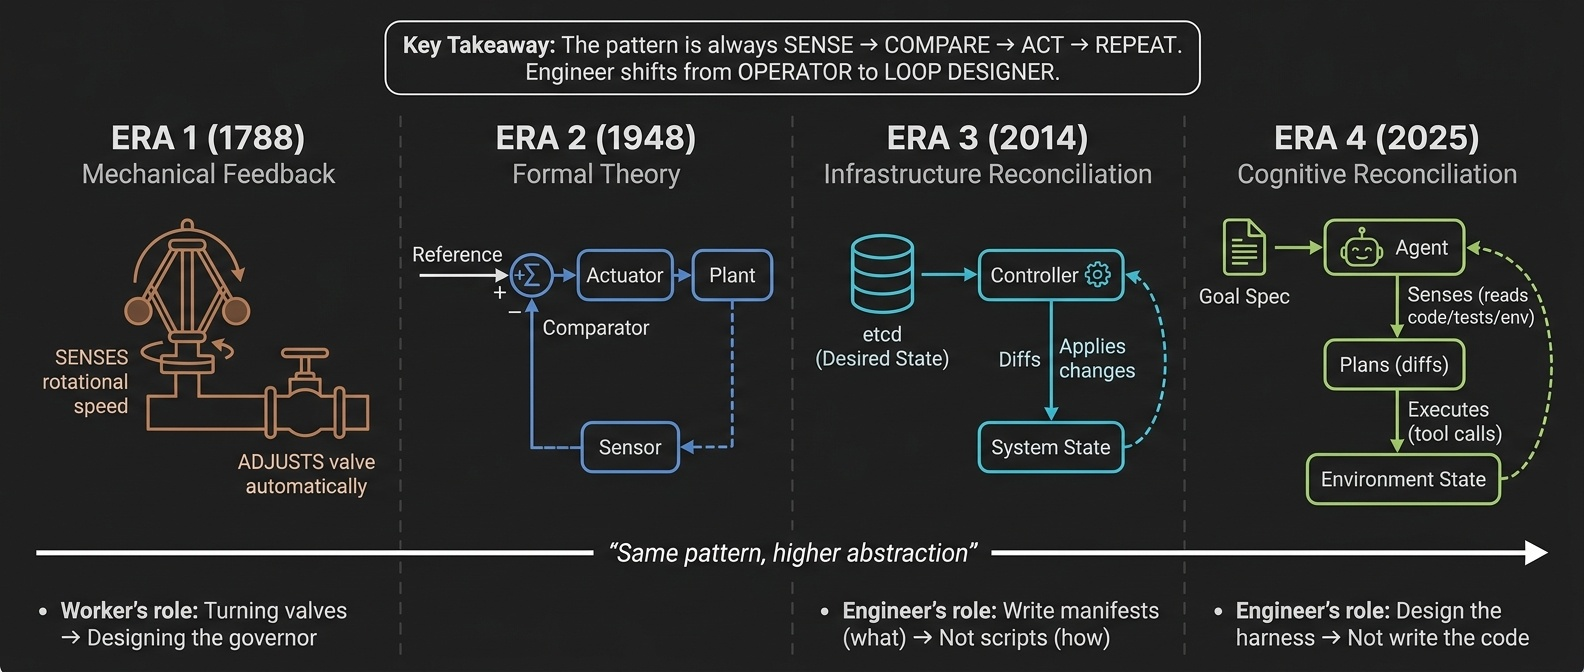
\includegraphics[width=0.9\linewidth]{pic/eras.png}
  \vspace{0.2cm}

  \small Each era moves the human \textbf{up one level}: from turning the valve to designing the governor.
\end{frame}

% =====================================================================
\section[Cybernetics]{Cybernetics in Ten Minutes}

\begin{frame}{Every feedback loop has the same four parts}
  \centering
  \begin{tikzpicture}[node distance=0.9cm]
    \node (sp) [lbl] {goal\\(setpoint)};
    \node (s) [sum, right=0.7cm of sp] {$\Sigma$};
    \node (a) [blk, right=of s] {Actuator\\\tiny makes a change};
    \node (p) [blk, right=of a] {The system\\\tiny engine, cluster, code};
    \node (o) [lbl, right=0.7cm of p] {actual\\state};
    \node (sn) [blk, below=0.7cm of a, xshift=1.4cm] {Sensor\\\tiny measures};
    \draw[flow] (sp) -- (s);
    \draw[flow] (s) -- node[lbl, above] {error} (a);
    \draw[flow] (a) -- (p);
    \draw[flow] (p) -- (o);
    \draw[flow] ($(p.east)+(0.35,0)$) |- (sn);
    \draw[flow] (sn) -| node[lbl, pos=0.85, left] {$-$} (s);
    \node[lbl, above=0.08cm of s] {comparator};
  \end{tikzpicture}

  \vspace{0.3cm}
  \footnotesize
  \begin{tabular}{lllll}
    \toprule
     & \textbf{Goal} & \textbf{Sensor} & \textbf{Comparator} & \textbf{Actuator} \\
    \midrule
    Watt governor (1788) & target speed & spinning balls & linkage & steam valve \\
    Thermostat & 21\,°C & thermometer & switch & furnace \\
    Kubernetes (2014) & YAML manifest & API server watch & controller diff & controller writes \\
    Agent loop (2025) & task spec + checks & tests, logs, browser & diff vs. goal & LLM edits code \\
    \bottomrule
  \end{tabular}
\end{frame}

\begin{frame}{How control loops fail: Maxwell, \emph{On Governors} (1868)}
  Governors on steam engines \alert{hunted}: they overshot, corrected, overshot again. Maxwell's paper on why is one of the founding texts of control theory.
  \vspace{0.3cm}

  \footnotesize
  \begin{tabular}{L{3.2cm}L{5cm}L{5.3cm}}
    \toprule
    \textbf{Control term} & \textbf{What it means} & \textbf{In an agent loop} \\
    \midrule
    Negative feedback & push against the error & undo a change that made things worse \\
    Damping & slow down after overshooting & smaller changes, wait longer after a miss \\
    Oscillation (hunting) & overshoot, correct, repeat & fix one test, break two, fix those\dots \\
    Steady-state error & settles short of the goal & stuck: the agent can't close the last gap \\
    Saturation limits & the valve only opens so far & caps on rounds, time and money \\
    \bottomrule
  \end{tabular}
\end{frame}

\begin{frame}{Ashby's Law: you can only control what you can sense}
  \begin{block}{Law of Requisite Variety (W. Ross Ashby, \emph{An Introduction to Cybernetics}, 1956)}
    Only variety can absorb variety: a regulator can only correct the disturbances it can tell apart.
  \end{block}
  \vspace{0.2cm}
  \begin{itemize}
    \item For an agent loop the \textbf{checks are the sensors}. The loop can never be better than its checks.
    \item A bug the tests can't see is a bug the loop will happily ship.
    \item Goodhart's law is the dark side: a measure that becomes a target stops being a good measure.
    \item The cheapest way for an agent to make a failing test pass is to \alert{edit the test}.
  \end{itemize}
  \vspace{0.2cm}
  \centering\textbf{Invest in sensing before you invest in smarter planning.}
\end{frame}

\begin{frame}{Who steers the steersman?}
  \begin{columns}[c]
    \begin{column}{0.55\textwidth}
      \begin{itemize}
        \item Second-order cybernetics: the observer is part of the system it observes.
        \item An agent that can touch its own sensors is grading its own homework.
        \item So split the loop:
          \begin{itemize}
            \item \textbf{Brain outside}: goal, checks, limits, undo
            \item \textbf{Hands inside}: edits and the code they run
          \end{itemize}
        \item The human moves up again: you design and tune the loop, the loop does the work.
      \end{itemize}
    \end{column}
    \begin{column}{0.4\textwidth}
      \centering
      \begin{tikzpicture}
        \node[blk, minimum width=3.4cm, minimum height=2.6cm, fill=tsinghua!6] (b) {};
        \node[font=\sffamily\scriptsize\bfseries, text=tsinghua, anchor=north] at (b.north) {Brain (host)};
        \node[blk, minimum width=2.6cm, minimum height=0.9cm, below=0.55cm of b.north] (h) {Hands (sandbox)\\\tiny agent edits, tests run};
        \node[font=\sffamily\tiny, anchor=south, align=center] at (b.south) {goal $\cdot$ checks $\cdot$ limits $\cdot$ undo};
        \node[lbl, below=0.25cm of b] {You: design and tune the loop};
      \end{tikzpicture}
    \end{column}
  \end{columns}
\end{frame}

% =====================================================================
\section[Kubernetes]{Kubernetes: Cybernetics for Infrastructure}

\begin{frame}{The reconciliation loop}
  \begin{columns}[T]
    \begin{column}{0.5\textwidth}
      \begin{enumerate}
        \item \textbf{Desired state}: a manifest says what should exist
        \item \textbf{Observe}: read the current state
        \item \textbf{Diff}: compare desired vs.\ actual
        \item \textbf{Act}: make the smallest change that closes the gap
        \item \textbf{Repeat}: forever
      \end{enumerate}
    \end{column}
    \begin{column}{0.45\textwidth}
      \begin{block}{Level-triggered, not edge-triggered}
        A controller reacts to \emph{what is true now}, not to the event that just happened. Missed an event? The next pass still sees the gap.
      \end{block}
    \end{column}
  \end{columns}
  \vspace{0.3cm}
  The controller never runs a script from A to B. It only knows how to make the \emph{next correction}. Kill a pod and it comes back: \alert{self-healing falls out of the loop}. Nobody writes a special case for it.
\end{frame}

\begin{frame}[fragile]{What a controller looks like (controller-runtime, sketch)}
\begin{lstlisting}[language=Go, morekeywords={func,return,if,var,nil,err}]
func (r *ModelReconciler) Reconcile(ctx context.Context,
        req ctrl.Request) (ctrl.Result, error) {
    var m mlv1.Model
    if err := r.Get(ctx, req.NamespacedName, &m); err != nil { // observe
        return ctrl.Result{}, client.IgnoreNotFound(err)
    }
    if m.Status.ServedVersion == m.Spec.Version {     // diff
        return ctrl.Result{}, nil                      // converged
    }
    if err := r.rolloutOneStep(ctx, &m); err != nil { // act: one step
        return ctrl.Result{}, err                      // retried, backoff
    }
    return ctrl.Result{RequeueAfter: 30 * time.Second}, nil // repeat
}
\end{lstlisting}
  \small A hypothetical \texttt{Model} resource. Note what's missing: no plan, no sequence of steps, no memory of the last run.
\end{frame}

\begin{frame}{The control plane, mapped}
  \centering
  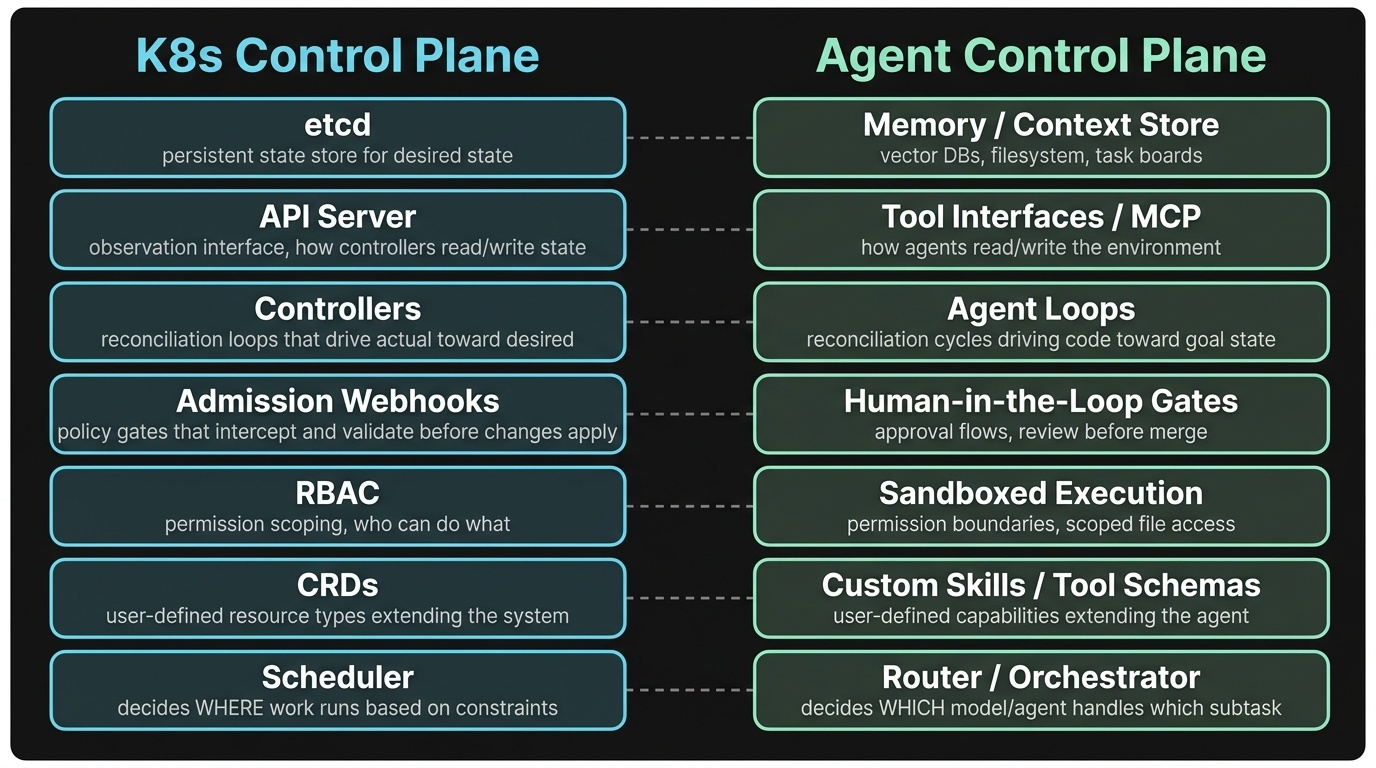
\includegraphics[width=0.82\linewidth]{pic/controlplane.png}
\end{frame}

\begin{frame}{MLOps already runs on these loops}
  \begin{itemize}
    \item \textbf{GitOps} (Argo CD, Flux): git holds the desired state, a controller syncs the cluster to it.
    \item \textbf{Continuous training}: a metric drops below the line, retrain until it's back above.
    \item \textbf{Progressive delivery}: canary metrics go bad, roll back automatically.
    \item \textbf{Data validation before training}: a gate that rejects bad input, like an admission webhook.
  \end{itemize}
  \vspace{0.4cm}
  \begin{block}{So what's new?}
    Only the actuator. The thing making the change is now a language model, and it can make \emph{any} change, including bad ones. Everything else you already know.
  \end{block}
\end{frame}

% =====================================================================
\section[Agent loops]{Agents: Same Machine, New Actuator}

\begin{frame}{Same loop, new actuator}
  \centering
  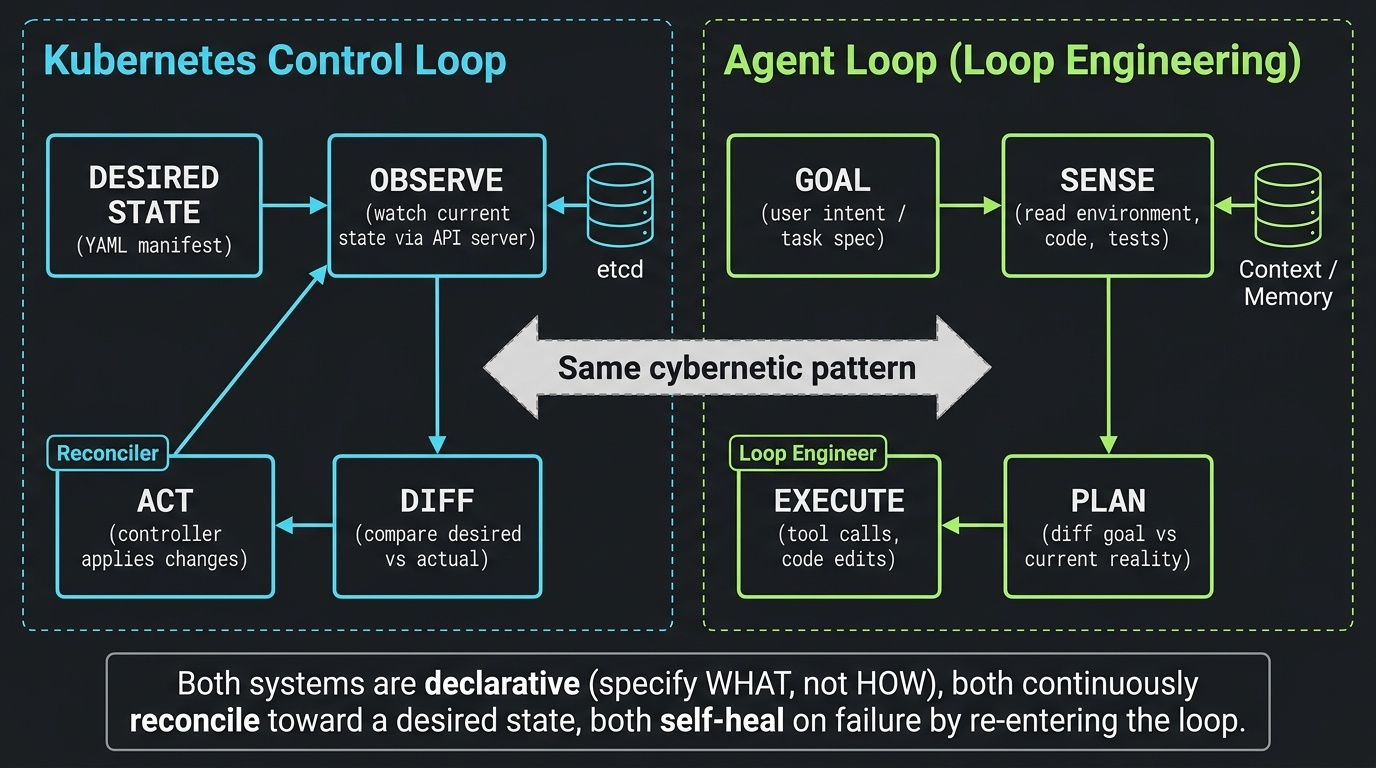
\includegraphics[width=0.78\linewidth]{pic/loops.png}
\end{frame}

\begin{frame}{Design rules that transfer directly}
  \footnotesize
  \begin{tabular}{L{2.8cm}L{5.2cm}L{5.6cm}}
    \toprule
    \textbf{Rule} & \textbf{In Kubernetes} & \textbf{In an agent loop} \\
    \midrule
    Declarative & manifest says \emph{what}, not \emph{how} & ``all checks pass'' beats a 47-step checklist \\
    Observe first & read the API server before acting & read the code and run the tests before editing \\
    Small diffs & change one thing per pass & one target per round, cap the diff size \\
    Idempotent & re-running a pass is harmless & ``file contains X'', not ``append Y'' \\
    Crash-only & controllers can die anytime & progress lives in git, not in the agent's head \\
    Bounded ownership & labels and selectors & one loop owns one directory \\
    \bottomrule
  \end{tabular}
\end{frame}

\begin{frame}[fragile]{Idempotency bit me while writing the demo}
  The scripted demo worker fixes one bug per run by replacing text in \texttt{calc.py}:
\begin{lstlisting}[language=Python]
# First version: replace the first `return a - b`
FIXES = {"add": ("return a - b", "return a + b"), ...}
# Run twice: once sub is fixed to `return a - b`, the add fix hits sub

# Fixed version: anchor on context, so a second run is a no-op
FIXES = {"add": ("def add(a, b):\n    return a - b",
                 "def add(a, b):\n    return a + b"), ...}
\end{lstlisting}
  \small ``Make the file \emph{contain} X'' converges. ``Do Y to the file'' drifts every time the loop re-runs it.
\end{frame}

% =====================================================================
\section[loopctl]{loopctl: The Loop, Built}

\begin{frame}{loopctl in one picture}
  \centering
  \begin{tikzpicture}[node distance=0.45cm]
    \node (obs) [blk, minimum width=1.6cm] {observe\\\tiny run checks};
    \node (dec) [blk, minimum width=1.6cm, right=of obs] {decide\\\tiny pick target};
    \node (act) [blk, minimum width=1.6cm, right=of dec] {act\\\tiny agent edits};
    \node (adm) [blk, minimum width=1.6cm, right=of act] {admit\\\tiny gates};
    \node (com) [blk, minimum width=1.6cm, right=of adm] {commit\\\tiny git};
    \node (ver) [blk, minimum width=1.6cm, right=of com] {verify\\\tiny re-observe};
    \foreach \a/\b in {obs/dec, dec/act, act/adm, adm/com, com/ver} \draw[flow] (\a) -- (\b);
    \draw[flow] (ver.south) -- ++(0,-0.5) -| node[lbl, pos=0.25, below] {repeat until every check passes or a breaker trips} (obs.south);
    \draw[flow, dashed] (ver.north) -- ++(0,0.45) -| node[lbl, pos=0.25, above] {broke a passing check: git revert} (com.north);
    \draw[flow, dashed] (adm.north) -- ++(0,0.45) -| node[lbl, pos=0.25, above] {rejected: discard} (act.north);
  \end{tikzpicture}

  \vspace{0.3cm}
  \small
  \begin{itemize}
    \item About 970 lines of Python, standard library only. Git is its etcd: every kept change is a commit.
    \item The agent is just a shell command. pi, Claude Code, Codex, or a script.
    \item Kill it at any point; rerun picks up where it left off, with budgets intact.
  \end{itemize}
\end{frame}

\begin{frame}[fragile]{The goal is a file}
\begin{lstlisting}[language=toml]
name  = "calc"
goal  = "calc.py arithmetic behaves as test_calc.py specifies."
actor = 'pi -p "$(cat)"'        # any agent CLI; the prompt arrives on stdin
fresh_clone = true               # observe a clean clone every round: no stale reads

[[checks]]                       # desired state = every check exits 0
name = "add"
run  = "python3 -m unittest -q test_calc.TestCalc.test_add"

[[admission]]                    # policy gate on every proposed change
name = "tests-unchanged"
run  = "git diff --cached --quiet -- test_calc.py"

[limits]                         # the safety governor
max_iterations = 10
max_diff_lines = 20              # damping: big changes are rejected
stall_iterations = 3             # steady-state error: give up
max_regressions = 2              # oscillation: stop thrashing
\end{lstlisting}
\end{frame}

\begin{frame}{Every part has a cybernetic name}
  \small
  \begin{tabular}{L{4.8cm}L{3.3cm}L{5.6cm}}
    \toprule
    \textbf{loopctl} & \textbf{Cybernetics} & \textbf{Kubernetes} \\
    \midrule
    \texttt{goal} + \texttt{[[checks]]} & setpoint & manifest \\
    running the checks & sensor & watch via API server \\
    passing vs.\ failing & comparator & diff \\
    the agent (\texttt{actor}) & actuator & controller writes \\
    \texttt{git revert} on regression & negative feedback & rollback \\
    backoff, \texttt{max\_diff\_lines} & damping & rate-limited requeue \\
    \texttt{max\_regressions} & oscillation guard & --- \\
    \texttt{stall\_iterations} & steady-state error & --- \\
    \texttt{[[admission]]}, approval & --- & admission webhooks \\
    lease file, sandbox & --- & RBAC, namespaces \\
    \texttt{[decider]} & controller logic & scheduler \\
    \bottomrule
  \end{tabular}
\end{frame}

\begin{frame}[fragile]{Demo 1: the loop converges (offline, scripted worker)}
\begin{lstlisting}[style=term]
$ ./examples/calc/demo.sh
[calc] observe: 1/4 passing, failing ['add', 'sub', 'div']
[calc] act #1: target `add`
[calc] committed 7f0e20ae (2 lines)
[calc] observe: 2/4 passing, failing ['sub', 'div']
[calc] act #2: target `sub`
[calc] committed c4470cd2 (2 lines)
[calc] observe: 3/4 passing, failing ['div']
[calc] act #3: target `div`
[calc] committed 7a07aa94 (2 lines)
[calc] observe: 4/4 passing
[calc] converged
\end{lstlisting}
  \small One target per round, observe after every change, stop when the sensors say done. Runs in about 2 seconds with no network.
\end{frame}

\begin{frame}[fragile]{Demo 2: a real agent as the actuator}
  \begin{columns}[T]
    \begin{column}{0.48\textwidth}
\begin{lstlisting}[language=toml]
actor = 'pi -p "$(cat)"'
\end{lstlisting}
\begin{lstlisting}[style=termsm]
$ ./examples/calc/demo.sh loop.pi.toml
...
[calc-pi] observe: 4/4 passing
[calc-pi] converged
calc-pi: 3 actions, 3 commits,
  0 rejected, 0 reverted, 23.6s acting
\end{lstlisting}
    \end{column}
    \begin{column}{0.48\textwidth}
      pi's fix for \texttt{div} was not the scripted one:
\begin{lstlisting}[style=termsm]
--- loop(calc-pi): #3 div
-    if b == 0:
-        return 0
\end{lstlisting}
      \small It deleted the guard so Python raises \texttt{ZeroDivisionError} itself. Different path, same goal. That's what ``declare \emph{what}, not \emph{how}'' buys you.
    \end{column}
  \end{columns}
\end{frame}

\begin{frame}[fragile]{Demo 3: brain outside, hands inside}
  \begin{columns}[T]
    \begin{column}{0.5\textwidth}
      Each check runs in a throwaway Apple container VM:
\begin{lstlisting}[language=bash, numbers=none]
container run --rm --network none \
  -v "$PWD":/work:ro -w /work \
  python:3.12-slim "$@"
\end{lstlisting}
\begin{lstlisting}[language=toml]
run = "./incvm python3 -m unittest ..."
\end{lstlisting}
    \end{column}
    \begin{column}{0.46\textwidth}
      What agent-written code sees inside:
\begin{lstlisting}[style=termsm]
home visible: False
network: blocked URLError
write /work: blocked Read-only file system
\end{lstlisting}
      \small loopctl and the agent stay on the host, so the agent can't rewrite how it's graded. About 1\,s per VM; the full loop converged in 55\,s.
    \end{column}
  \end{columns}
\end{frame}

% =====================================================================
\section[Failure modes]{When Loops Go Wrong}

\begin{frame}{Kubernetes already learned these lessons}
  \footnotesize
  \begin{tabular}{L{2.6cm}L{4.4cm}L{6.4cm}}
    \toprule
    \textbf{Failure} & \textbf{Looks like} & \textbf{loopctl's answer} \\
    \midrule
    Thrashing & fix one test, break two & verify every commit; revert on regression; stop after \texttt{max\_regressions} \\
    Stale reads & acting on an old picture & re-run checks every round, optionally on a fresh clone \\
    Endless loop & goal can't be reached & caps on rounds and time; \texttt{stall\_iterations} \\
    Fighting loops & two loops, one directory & lease file; edits outside the directory halt the loop \\
    Gaming the sensor & agent edits the test & admission checks reject the change \\
    Blind loop & no signal to steer by & nothing to fix in the loop: add checks \\
    \bottomrule
  \end{tabular}
\end{frame}

\begin{frame}[fragile]{Live failure: thrashing gets caught}
  A worker that fixes \texttt{add} but breaks \texttt{mul} every time:
\begin{lstlisting}[style=term]
[calc] observe: 1/4 passing, failing ['add', 'sub', 'div']
[calc] act #1: target `add`
[calc] committed 84dcb427 (4 lines)
[calc] observe: 1/4 passing, failing ['sub', 'mul', 'div']
[calc] reverted 84dcb427: broke ['mul']
[calc] act #2: target `add`
[calc] committed 8a047e50 (4 lines)
[calc] observe: 1/4 passing, failing ['sub', 'mul', 'div']
[calc] reverted 8a047e50: broke ['mul']
[calc] thrashing: 2 reverted regressions
\end{lstlisting}
  \small Negative feedback (revert), then a hard stop instead of hunting forever. Every attempt stays in git history for a human to read.
\end{frame}

\begin{frame}[fragile]{Live failure: the agent tries to move the goalposts}
  A worker that ``fixes'' \texttt{add} by changing the expected answer in the test:
\begin{lstlisting}[style=term]
[calc] act #1: target `add`
[calc] rejected: admission[tests-unchanged]: exit 1
...
[calc] unreachable: no progress in 3 iterations; still failing ['add', 'sub', 'div']
\end{lstlisting}
  \vspace{0.2cm}
  \begin{itemize}
    \item Goodhart's law, blocked by an admission webhook: one line of shell.
    \item The loop gives up instead of shipping a fake green build.
    \item \texttt{loopctl report} shows the pattern: 3 rejections, all \texttt{admission[tests-unchanged]}.
  \end{itemize}
\end{frame}

% =====================================================================
\section[Decider]{A Small Brain That Decides}

\begin{frame}{The scheduler doesn't run pods. It picks.}
  \begin{columns}[T]
    \begin{column}{0.5\textwidth}
      \textbf{Kubernetes scheduler}
      \begin{itemize}
        \item filter: which nodes \emph{can} run this pod?
        \item score: which is best?
        \item pick one; the kubelet does the work
      \end{itemize}
      \vspace{0.2cm}
      \textbf{Same split for agents}
      \begin{itemize}
        \item a small, fast model \textbf{decides}
        \item a big, slow model \textbf{does}
        \item the checks \textbf{judge}
      \end{itemize}
    \end{column}
    \begin{column}{0.46\textwidth}
      \begin{block}{TypeSafe Jev}
        Answers typed questions with probabilities instead of free text. One request per round:
        \begin{itemize}
          \item move: act / ask a human / stop
          \item target: which failing check next
        \end{itemize}
      \end{block}
    \end{column}
  \end{columns}
\end{frame}

\begin{frame}{What the decider is not allowed to do}
  \begin{itemize}
    \item \textbf{Judge.} It can't mark anything as passed. Only the checks converge the loop.
    \item \textbf{Pick outside the menu.} A passing check as target is rejected; that round uses the built-in rule.
    \item \textbf{Act on a shaky call.} Under 50\% confidence, or ``ask a human'': loopctl stops and asks.
    \item \textbf{Override the governor.} Caps on rounds, time, thrashing and stalling still apply.
    \item \textbf{Break the loop.} If it crashes or times out, the loop falls back to the simple rule.
  \end{itemize}
  \vspace{0.3cm}
  \centering\small Typed output guarantees the \emph{shape} of the answer, not that it's right. Keep the judge outside.
\end{frame}

\begin{frame}[fragile]{Rules vs.\ Jev: an impossible check listed first}
  \texttt{gpu} runs \texttt{nvidia-smi}: no code change can make it pass on a Mac.
  \begin{columns}[T]
    \begin{column}{0.37\textwidth}
      \textbf{Built-in rule} (first failing check)
\begin{lstlisting}[style=termsm]
act #1: target `gpu`
rejected: no_op: actor made no changes
act #2: target `gpu`
rejected: no_op: actor made no changes
act #3: target `gpu`
rejected: no_op: actor made no changes
unreachable: no progress in 3 iterations
\end{lstlisting}
      \small\alert{0 of 3 fixable checks fixed.}
    \end{column}
    \begin{column}{0.61\textwidth}
      \textbf{Jev decider}
\begin{lstlisting}[style=termsm]
decide: act `add` (0.98)
  target add=0.67 div=0.22 sub=0.09 gpu=0.02
committed 22ef9645
decide: act `sub` (0.98)
  target sub=0.90 div=0.10 gpu=0.00
committed 6f7b3f5c
decide: act `div` (0.96)
  target div=1.00 gpu=0.00
committed 3d5f5a34
decide: stop `gpu` (0.97)
  stop=0.99 ask_human=0.01 act=0.00
unreachable: decider chose stop
\end{lstlisting}
      \small\textbf{3 of 3 fixed}, then stopped by itself. Whole run: about 3\,s.
    \end{column}
  \end{columns}
\end{frame}

% =====================================================================
\section[Outer loop]{The Loop Above the Loop}

\begin{frame}[fragile]{The hill-climbing machine}
  \begin{columns}[T]
    \begin{column}{0.48\textwidth}
      The same loop, one level up:
      \begin{enumerate}
        \item ship a v0 agent
        \item record what it does (traces)
        \item mine traces for failure patterns
        \item turn failures into checks
        \item improve the agent; repeat
      \end{enumerate}
      \small The setpoint is now \emph{agent quality}. You are the actuator.
    \end{column}
    \begin{column}{0.5\textwidth}
\begin{lstlisting}[style=termsm]
$ loopctl report loop.jev.toml
calc-jev: 3 actions, 3 commits, 0 rejected,
  0 reverted, 0.1s acting
last outcome: unreachable (decider chose stop)

checks observed failing:
     4  gpu
     3  div
     2  sub
     1  add

decisions:
     3  decider: act
     1  decider: stop
\end{lstlisting}
    \end{column}
  \end{columns}
\end{frame}

\begin{frame}[fragile]{Your turn (5 min): write the loop for a model}
  \begin{columns}[T]
    \begin{column}{0.55\textwidth}
\begin{lstlisting}[language=toml, basicstyle=\ttfamily\scriptsize, numbers=none]
name  = "churn-model"
goal  = "The churn model is fit to ship."
actor = 'pi -p "$(cat)"'

[[checks]]
name = "schema"     # data contract holds
run  = "python validate.py data/train.parquet"
[[checks]]
name = "quality"    # setpoint on a metric
run  = "python eval.py --min-auc 0.85"

[[admission]]
name = "holdout-untouched"
run  = "git diff --cached --quiet -- eval.py data/holdout/"
\end{lstlisting}
    \end{column}
    \begin{column}{0.42\textwidth}
      With your neighbour:
      \begin{enumerate}
        \item If \emph{you} were the agent, how would you cheat these checks?
        \item What could go wrong that no check here can see? (Ashby)
        \item When should this loop stop and ask a human?
        \item Which limit would you set first?
      \end{enumerate}
    \end{column}
  \end{columns}
\end{frame}

\begin{frame}{Takeaways}
  \begin{enumerate}
    \item \textbf{Declare the exit condition, not the path.} Checks are your setpoint.
    \item \textbf{Your checks are your sensors.} The loop is only as good as what it can see.
    \item \textbf{Never let the actuator touch the sensor.} Brain outside, hands inside.
    \item \textbf{Observe before every action.} Don't trust the agent's memory.
    \item \textbf{One small change per round, verified.} Undo anything that makes it worse.
    \item \textbf{Keep actions safe to repeat, and state outside the agent.} Then you can kill it anytime.
    \item \textbf{Install a governor.} Caps on rounds, time and money, plus a human gate.
    \item \textbf{Let a small model decide and a big model do.} The checks still judge.
  \end{enumerate}
  \vspace{0.2cm}
  \centering\textit{This isn't new. It's Kubernetes for thinking, and Watt's governor for software.}
\end{frame}

\begin{frame}{Further reading}
  \small
  \begin{itemize}
    \item S. Das, \href{https://blog.ucalyptus.me/p/loop-engineering-is-just-k8s-style}{\emph{Loop Engineering Is Just K8s-Style Orchestration}} (blog.ucalyptus.me)
    \item N. Wiener, \emph{Cybernetics: Or Control and Communication in the Animal and the Machine}, 1948
    \item W. R. Ashby, \emph{An Introduction to Cybernetics}, 1956
    \item J. C. Maxwell, \emph{On Governors}, Proceedings of the Royal Society, 1868
    \item \href{https://github.com/kubernetes-sigs/controller-runtime}{controller-runtime} and the \href{https://kubernetes.io/docs/concepts/scheduling-eviction/kube-scheduler/}{Kubernetes scheduler} docs
    \item \href{https://github.com/apple/container}{Apple container} and \href{https://github.com/ucalyptus/pi-cvm}{pi-cvm} (github.com/ucalyptus/pi-cvm)
    \item \href{https://docs.typesafe.ai}{TypeSafe docs} (docs.typesafe.ai)
  \end{itemize}
\end{frame}

\begin{frame}
\begin{center}
	{\Huge\calligra Thanks!}
\end{center}
\end{frame}

\end{document}
